\documentclass[12pt]{article}
\usepackage[hmargin=1in, vmargin=1in]{geometry}
\usepackage{fancyhdr}
\pagestyle{fancy}
\usepackage[hang,small]{caption}
\usepackage{lastpage}
\usepackage{graphicx}
\usepackage{verbatim}
\DeclareGraphicsExtensions{.jpg}
\usepackage{url}

\def\author{Jacques Uber}
\def\title{Technical Description: FredMeyer Camping Headlamp}
\def\date{\today}

\fancyhf{} % clear all header and footer fields
\fancyhead[LO]{\author}
\fancyhead[RO]{\date}
% The weird spacing here is to get the spacing of \thepage to be right.
\fancyfoot[C]{\thepage\
                    / 6}

\setcounter{secnumdepth}{0}
\setlength{\parindent}{0pt}
\setlength{\parskip}{4mm}
\linespread{1.4}
% Talk about how the hinge works and where the power switch it relative to how the hinge swings.
% Pictures:
%   Use copyright: Name, Year
% Get rid of value language
%
% OO: Wednesday 9-12
%
\begin{document}
\fancyhead[CO]{\title}
\listoffigures
\listoftables
\section{Introduction}
\begin{comment}
Questions:
*   How should you reference figures and tables in a sentence?
*   What should be in my conclusion?
*   Two or one space after a period?

Introduction:
    "This is what is going on in the paper"

Background:
    "Context" -- Know who your audience is.
    Talk about things outside of the individual object.

Note: You can combine the Into. and Background in this paper.

Body:
    Descriptions of characteristics
    Functions
    Descriptions of related processes

Conclusion:
    "What I need from you"

Formatting
----------
        Title
        -----
Introduction
++++++++++++
Names the object.
Context
Overview
Contents of descriptiong

Body
++++
Characteristics
Components
Materials
Functions

\end{comment}
The FredMeyer headlamp is a pocket sized light source designed for wearing around a user's head during
situations when visibility could be aided by a supplementary light source.

The headlamp is made up of two physical parts: a black lamp containing 6 LEDs (Light Emitting
Diodes), and a black elastic variable-length strap. The lamp has three settings allowing for light
of different color to be emitted from the LEDs. This paper describes the lamp, strap, and power
settings.

\begin{figure}[h!]
\centering
\caption[Front view of the headlamp] {Front view of the headlamp. \copyright Jacques Uber 2012}
\label{fig:DERP}
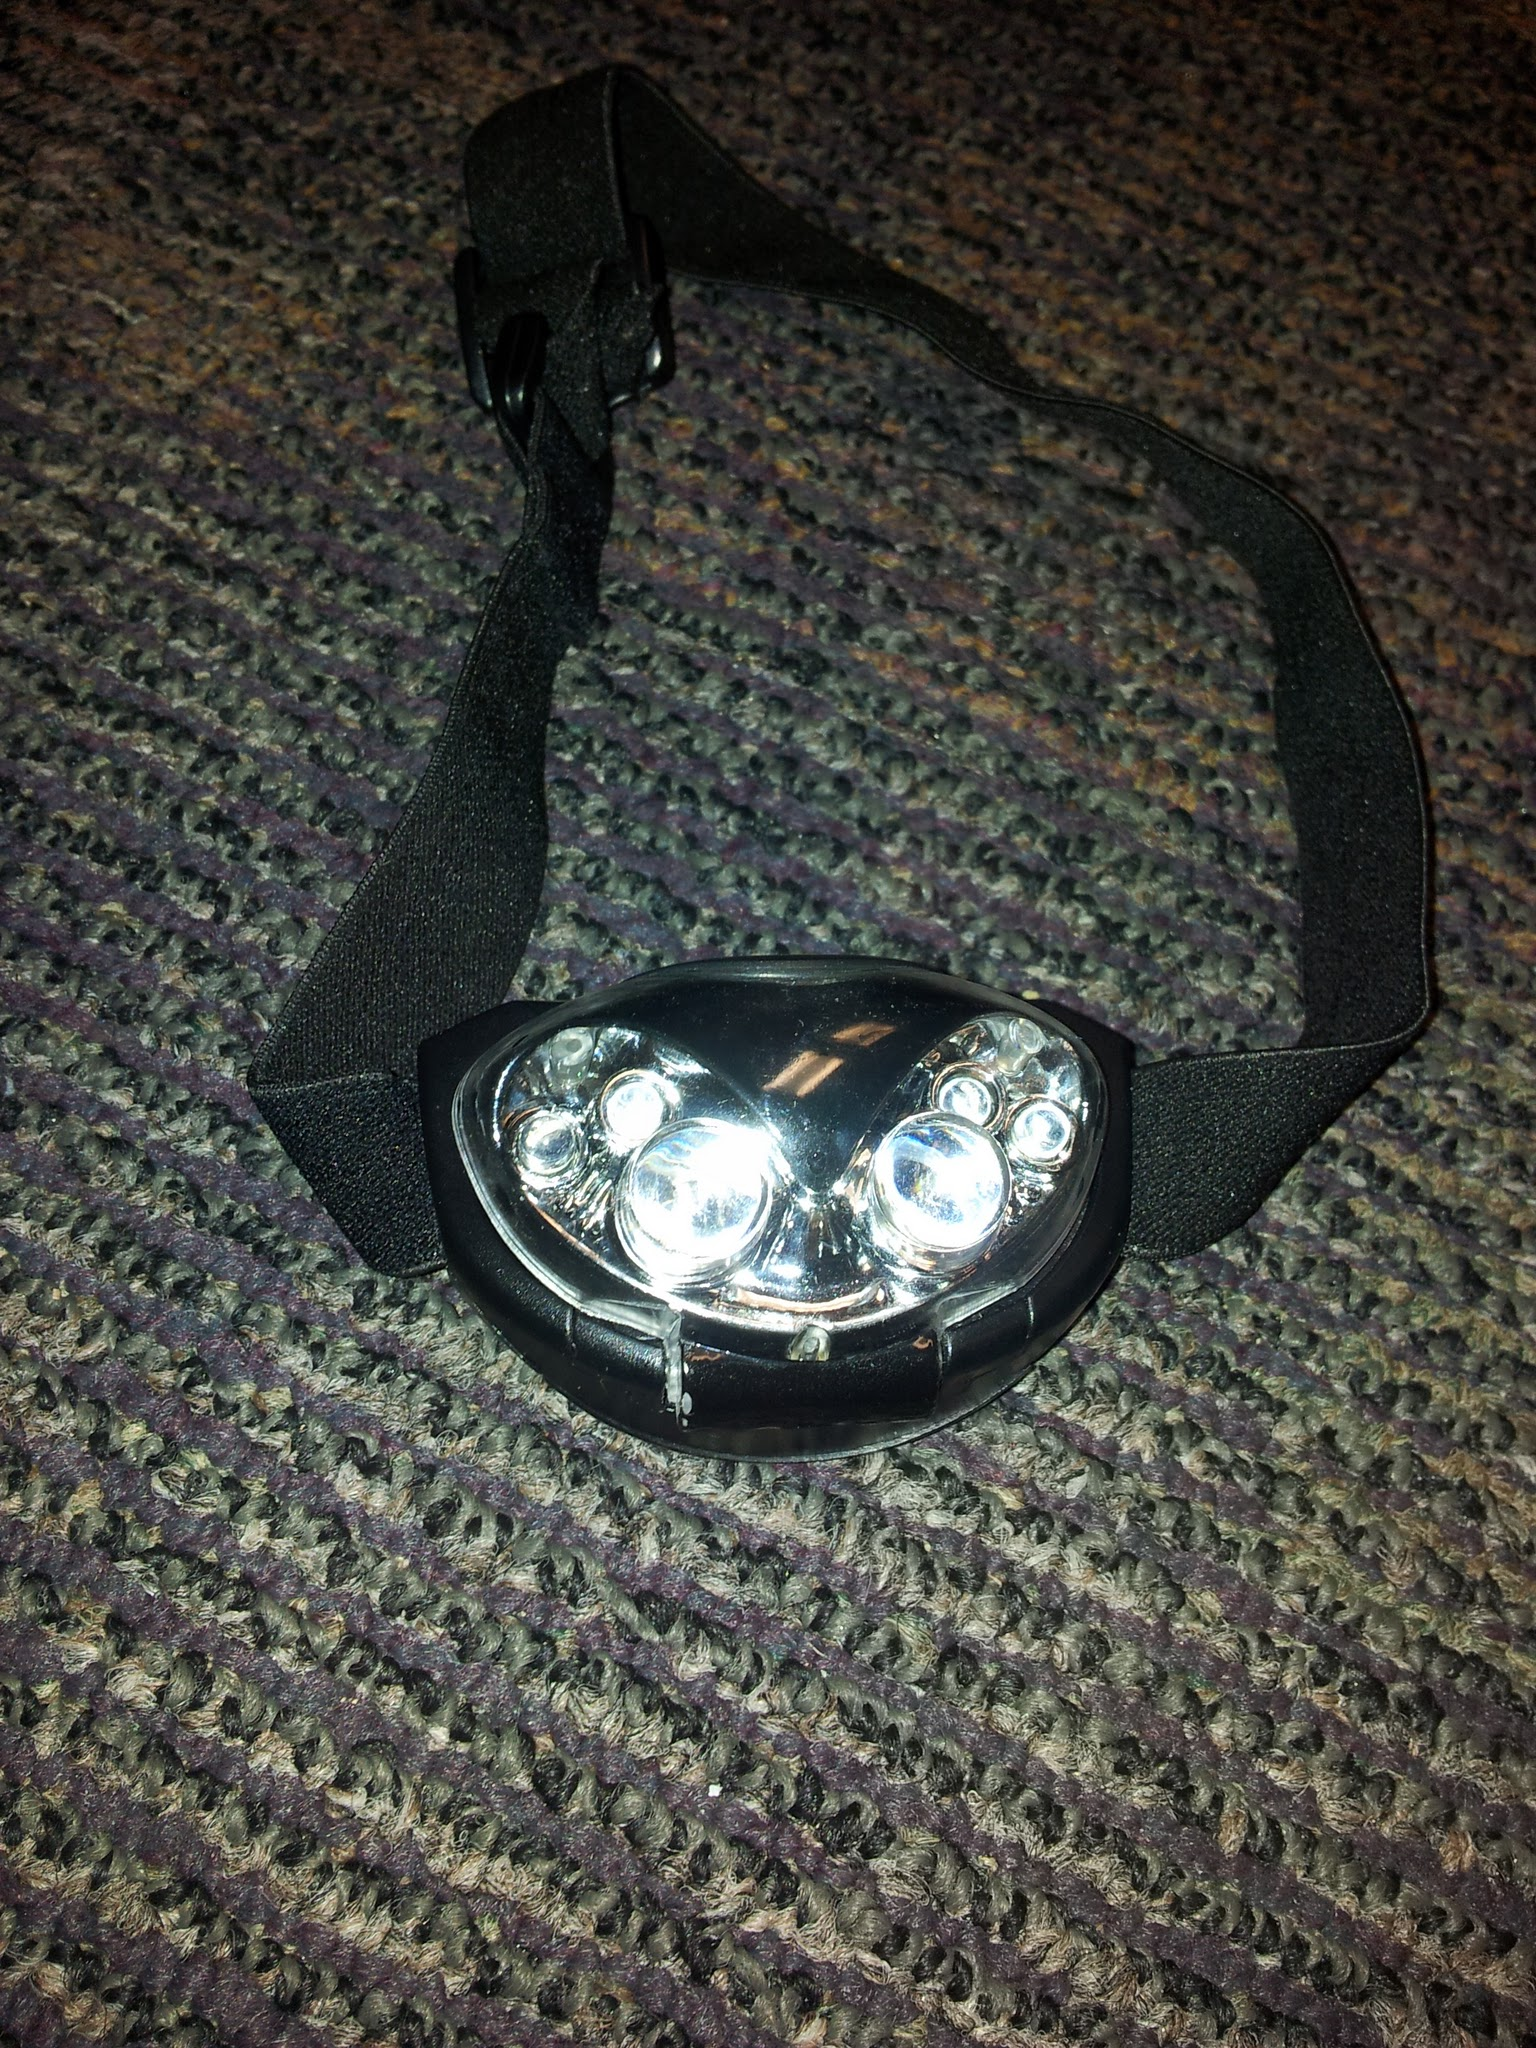
\includegraphics[width=3in]{headlamp}
\end{figure}

\begin{figure}[h!]
\centering
\caption[Side view of the headlamp] {Side view of the headlamp. \copyright Jacques Uber 2012}
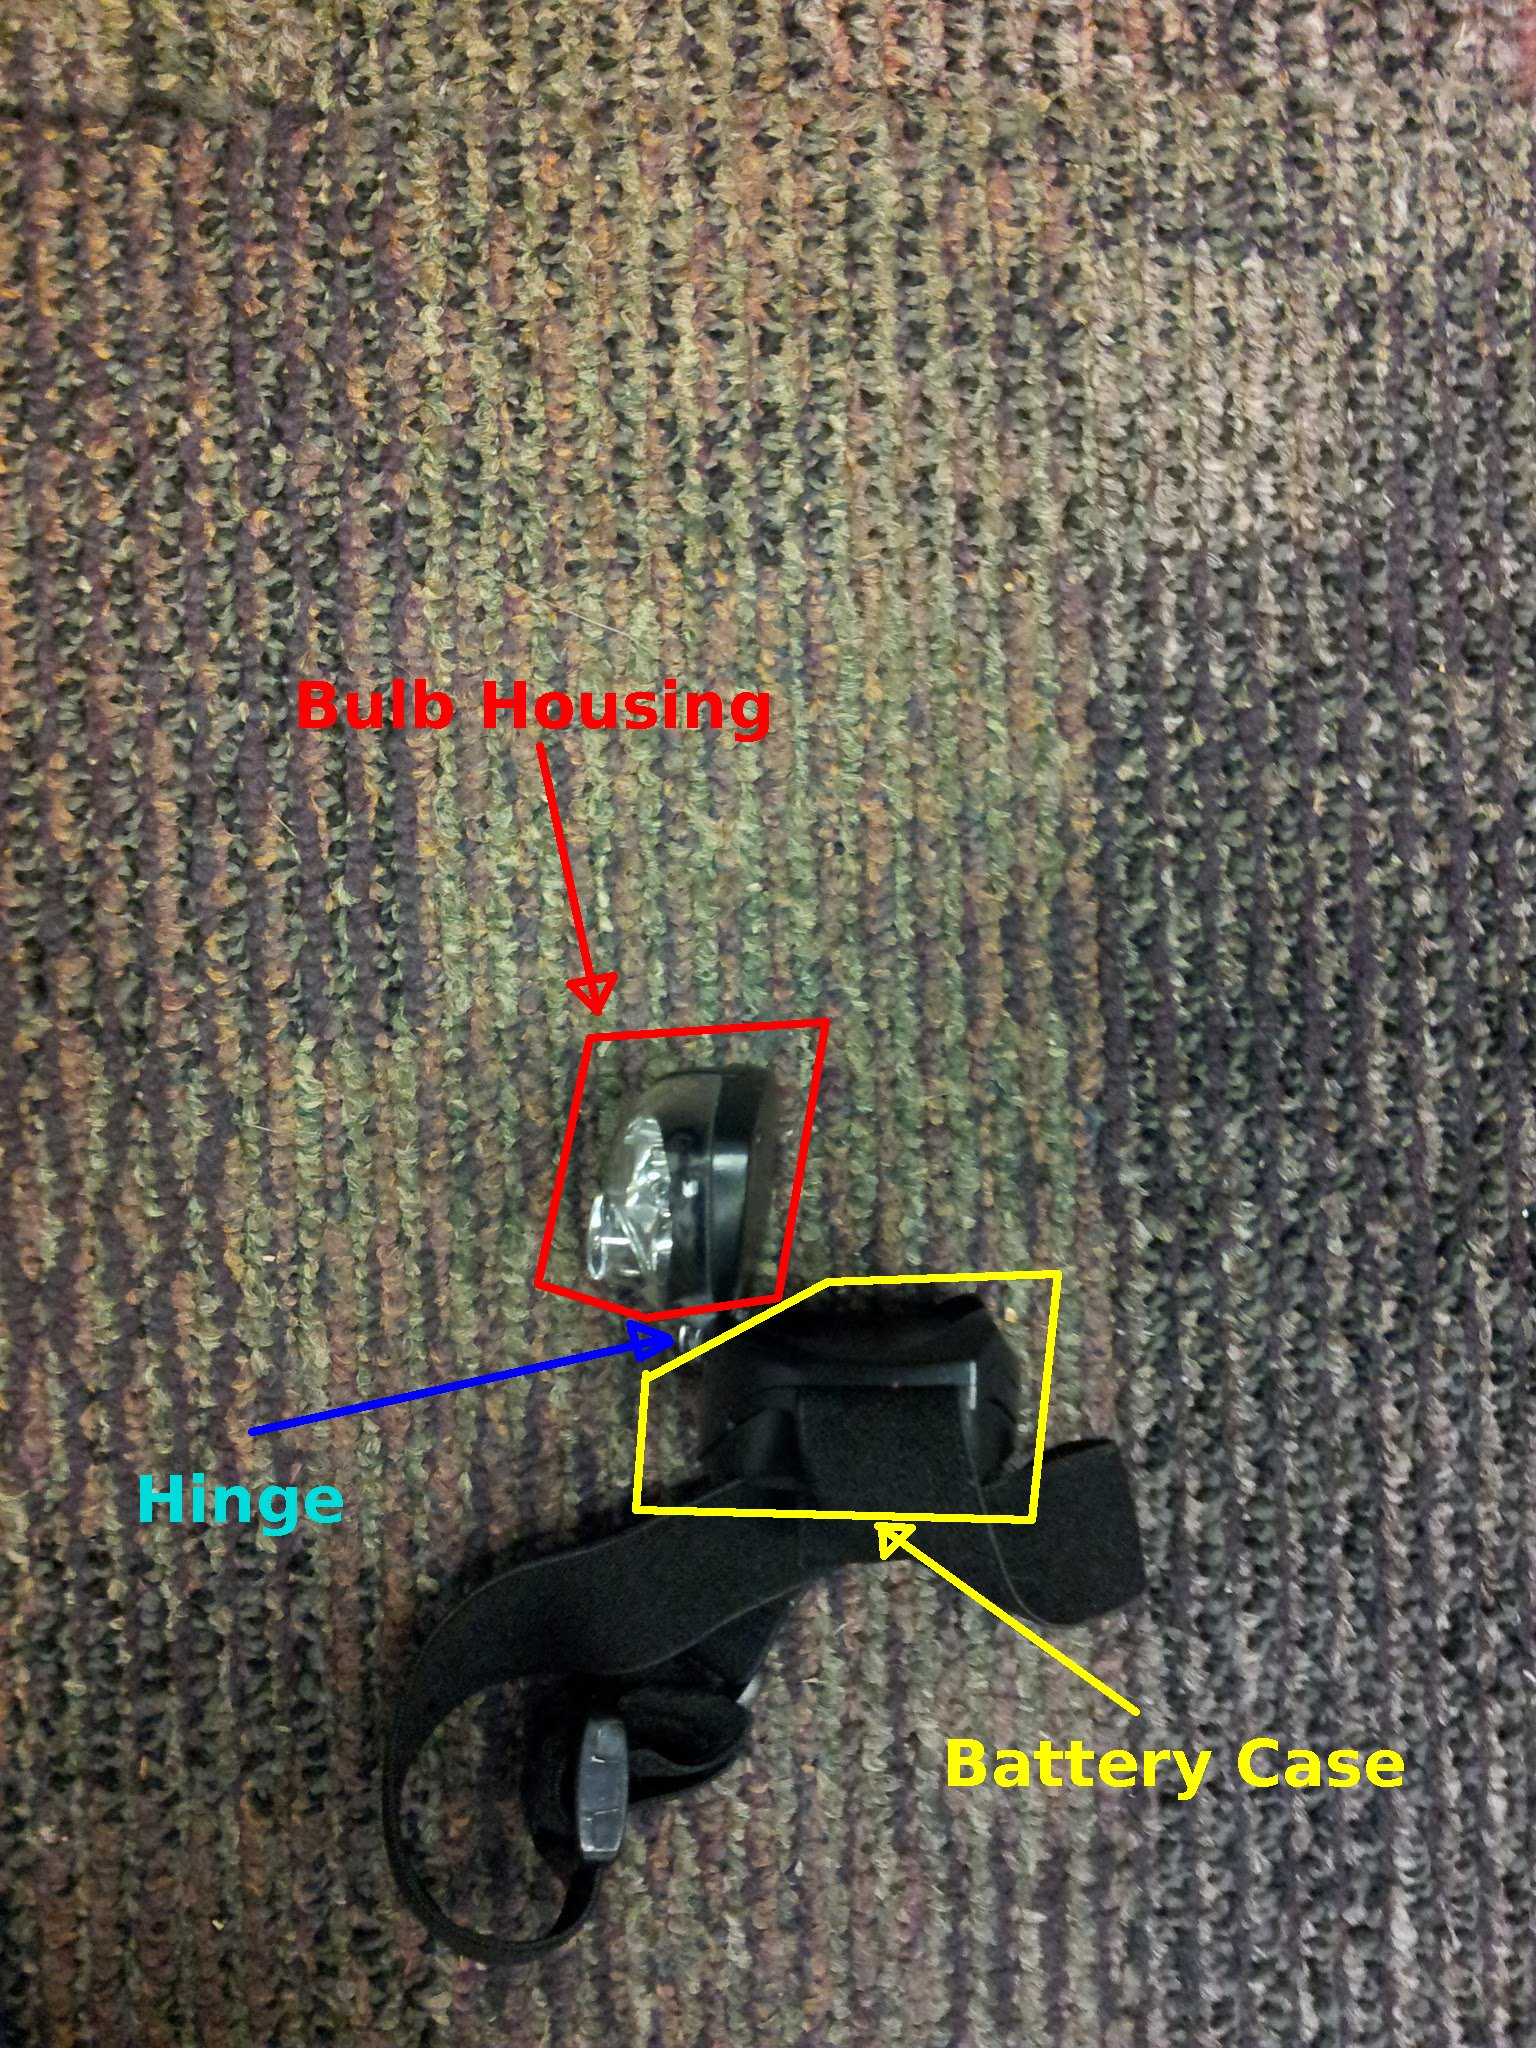
\includegraphics[width=3in]{headlamp_side}
\end{figure}

\begin{figure}[h!]
\centering
\caption[Top view of the headlamp] {Top view of the headlamp. \copyright Jacques Uber 2012}
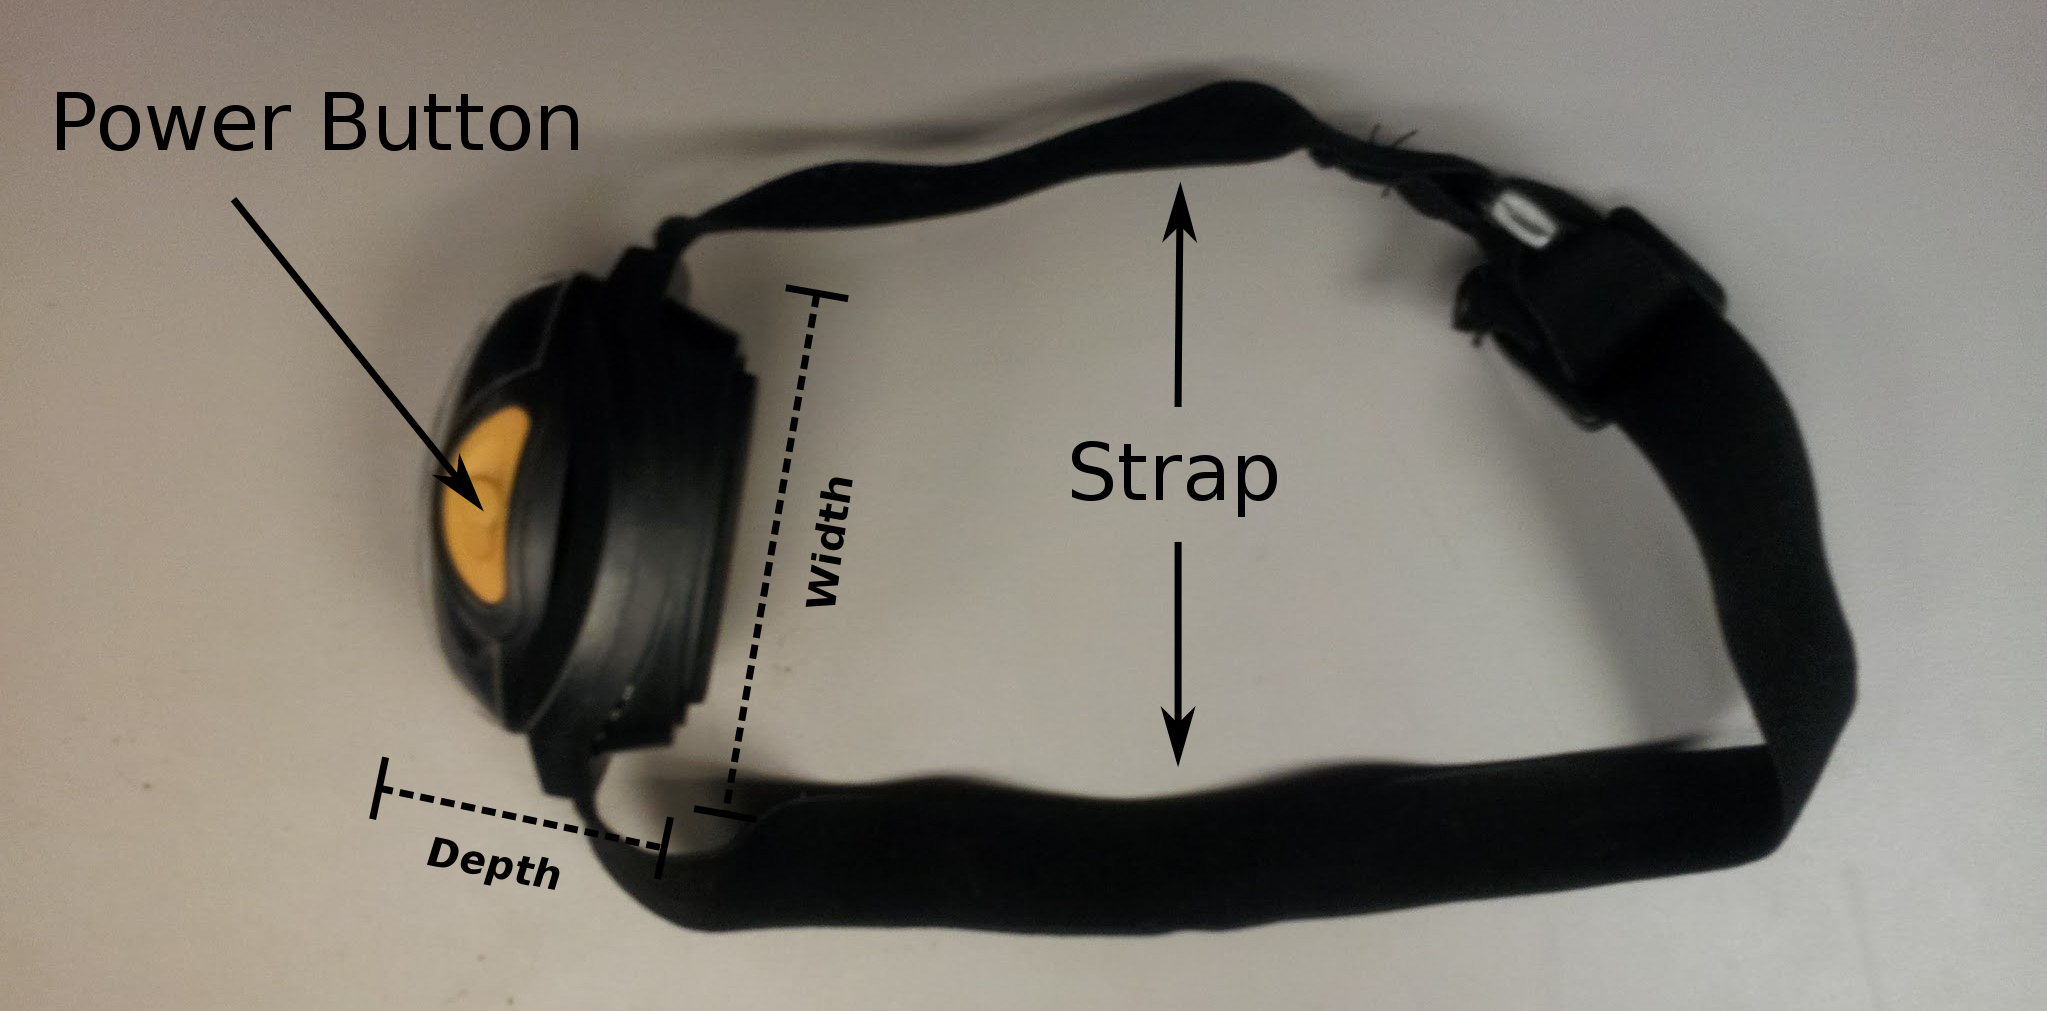
\includegraphics[width=3in]{headlamp_top}
\end{figure}

\section{The Lamp}
The lamp preforms the primary function of the headlamp. It is 1/4 pounds when loaded with
it's 3 AAA battery power source. The lamp itself is split into two modules: the LED housing and the
battery case. The two modules are joined by a hinge which allows the LEDs to be aimed variably (see
figure 2).

\begin{table}
\begin{center}
\begin{tabular}{ | c | c | c | p{5cm} |}
    \hline
    Height & Width & Depth \\ \hline
    3cm & 5cm & 2.5cm  \\ \hline
\end{tabular}
\end{center}
\caption{Lamp Dimensions}
\end{table}

\subsection{LED housing}
The LED housing module holds the LEDs, LED casing, and power switch.

\subsubsection{LEDs}
The lamp has 6 main LEDs, 4 of the LEDs are white and the remaining 2 are red. Of the 4 white LED's
2 of them have a radius of 0.5cm and are located symmetrically opposite of each other located 1cm
away from the front center line of the lamp.  The remaining 4 LEDs have a radius of 0.25cm and are
aligned symmetrically opposite to each other and are lined up starting 2cm away from the front
center line of the lamp. With regard to the 4 0.5cm LEDs, the two furthest from the center line are
white, the inner pair are red (see figure 1).

\subsubsection{LED Casing}
To protect the LEDs, a clear form fitting case covers the front of the lamp.  The case also acts to
focus and intensify the light from the LEDs. The case consists of hard plastic and is roughly
3mm thick.

\subsubsection{Power Toggle}
Turning on the lamp and cycling through the lamp's power settings is done with the plastic yellow
power toggle located on the top of the lamp (see figure 3). The toggle is pressure sensitive.

\subsection{Battery Case}
The majority of the headlamp is used to house the power supply. The supply case is rectangular with
rounded edges (see figure 2). It is 5cm across, 3cm wide, and 1.5cm deep. When in use, the back of
the case is placed on to the users forehead. To make this more comfortable there is a soft black
padding on the back 5cm by 3cm panel.

\section{The Strap}
The strap serves the function of holding the headlamp to the users head. The variable-length strap
is at maximum 2 feet long, and at minimum 1/2 foot long (see figure 3). It is made of an elastic material that
is black. The elasticity of the strap allows a strip of contracted material to be stretched into a
strip 2 times it's original length.
\begin{table}
\begin{center}
\begin{tabular}{ | c | c | c | p{5cm} |}
    \hline
    Height & Thickness & Length \\ \hline
    1.5cm & 2.5mm & 2ft  \\ \hline
\end{tabular}
\end{center}
\caption[Strap Dimensions]{Strap Dimensions when the strap is fully extended.}

\end{table}

\section{LED settings}
The LEDs can be configured via the power toggle to emit three forms of light: Normal-White,
Bright-White, and Flashing-Red (see table 3). These settings are achieved by powering some LEDs while not
powering others.

\begin{table}
\begin{center}
\begin{tabular}{ | c | c | c | p{5cm} |}
    \hline
    State & State Offset & \# of Powered LEDs & Description \\ \hline
    Normal White & 1 & 2 &  Baic setting. Two main LEDs are powered. Most appropriate for use over
    long time durations.\\ \hline
    Bright White & 2 & 4 &  Brightest setting. Two main LEDs and two white auxilary LEDs powered.
    Most appropriate setting when a very bright light is needed.\\ \hline
    Flashing Red & 3 & 4 &  Highest contrast setting. Two red auxilary LEDs flash.\\ \hline
\end{tabular}
\end{center}
\caption[Lamp Power States] {Headlamp states. State Offset refers to the offset (number of power toggles) from the 'off' state.}
\end{table}

\subsection{Normal-White}
From the off state, toggling power once will place the headlamp into the Normal-White state.  This
setting drives power to the two main, 0.5cm radius, LEDs.

\subsection{Bright-White}
From the off state, toggling power twice will place the headlamp into the Bright-White state.  This
setting drives power to both the two main, 0.5cm radius, LEDs and the two outer white, 0.25cm
radius, LEDs. The headlamp emits the most light while in this state.

\subsection{Flashing-Red}
From the off state, toggling power three times will place the headlamp into the Flashing-Red state.
This setting drives power to the two inner, 0.5cm radius, red LEDs. While in this state the
LEDs will flash on and off at a frequency of 3 times per second. Each flash has a duration of
0.25 seconds.


\end{document}
